\subsection{Background}
The Corporate Partnership Programme is a website designed to `promote the relationship between the Department of Computing and organisations who wish to recruit our students whilst investing in academic sponsorship'\cite{doc-cpp}.

In order for students to use the system they must log on, register some tick box interests, and then upload their CV.
For the student once they have done this their CPP journey is complete.
Corporate Partners then log on and can browse this list of students in order to contact them regarding internships, placements, and graduate opportunities. Of course they can send emails too, but this is done by sending an email to the CPP administrators when they can then forward on if deemed fit for purpose.

\begin{figure}[H]\centering
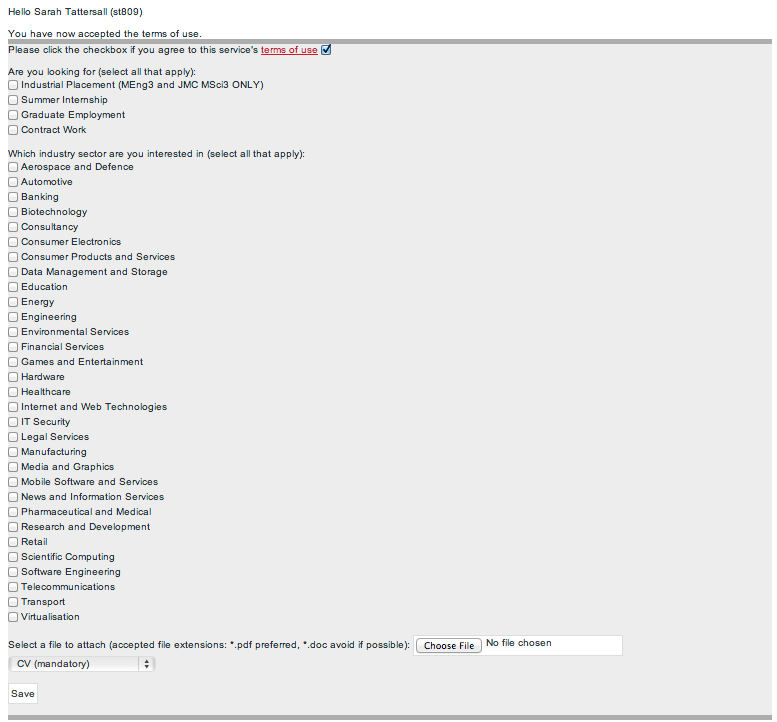
\includegraphics[scale=0.5]{images/introduction/old_cpp}
\caption{Entirety of the old site as viewable to the student}
\end{figure}
